\chapter{Introduction}

Thirty-nine percent of humans live within 100 km of a coast, and many of the world's largest cities are located in coastal areas \parencite{Magdalena2021}. Further, 10\% of all human beings live in zones less than 10m above sea level, an area known as the Low Elevation Coastal Zone (LECZ) \parencite{Neumann2015,Lichter2011}. These economically and socially important areas are under significant stress due to anthropogenic climate change and the consequent sea level rise (SLR). Changing climate patterns will likely create more intense storms, which combined with a higher sea level boundary condition due to SLR, puts these populations and infrastructure investments at significant risk. Additionally, climate change can increase water stress and result in increases in groundwater abstraction, leading to subsidence of coastal areas. Climate change presents severe, even existential risks for coastal zones and those who inhabit them.

To mitigate these risks economically, substantial research into coastal protection strategies and climate adaptation measures is required. Scientific research will help fully quantify the risks, allow better prioritization of mitigation efforts, and help develop strategies for climate adaptation and coastal protection that work in harmony with nature. A critical variable for this research is nearshore bathymetric data \parencite{Holman2013}, which allows mapping of the spatial extents of flooding and better quantification of the wave transformation on the coasts. 

However, this critical data is often missing in most of the world, due to the complication and expense of surveying it. This project aims to capitalize on recent advances in remote sensing technology to explore ways of improving current bathymetry estimates without requiring any in-situ data. 

\section{Motivation and Relevance}
\subsection{Importance of Nearshore Bathymetric Data}

Bathymetric data is essential for many aspects of the blue economy, including aquaculture, marine energy, submarine cables, dredging operations, design of sea defenses, navigation, ecosystem preservation, and as a boundary condition for numerical studies of wave transformation. \parencite{Cesbron2021,Ashphaq2021}. However, the nearshore zone is notoriously difficult to survey. There is currently a global lack of data in the 5-10~m zone \parencite{Albright2021} and up to 50\% of the world's shallow coastal zones remain unsurveyed \parencite{IHO/OHI2022}. Where surveys do exist, they can be decades out of date, especially in the 40\% of the world's coasts that are sandy and highly dynamic \parencite{Almar2021e}.

There have been attempts at global bathymetric datasets, most notably the General Bathymetric Chart of the Ocean (GEBCO), which is an annually-updated global bathymetric and topographic dataset. The bathymetry in GEBCO grids is derived by assimilation many different types of historic data, including  acoustic soundings provided by ships and gravimetric bathymetry measurements \parencite{Cesbron2021}. While it provides useful information about deep oceans, GEBCO accuracy in the nearshore zone is limited because sonar data is limited in many shallow nearshore zones. \parencite{Monteys2015}. Additionally, the horizontal and vertical resolution is not sufficient for accurate numerical studies of wave modeling. Bathymetric data with sufficient resolution for coastal wave modeling is available in most of the United States from NOAA, and most of the European Union via EMODnet. Outside these regions, there is little to no high-resolution bathymetric data. 

\subsection{Satellite-derived bathymetry}

Because of the difficulty of directly measuring bathymetry, there have been many attempts to find ways to estimate bathymetry based on remote sensing satellite data. There are two broad types of Satellite-Derived bathymetry (SDB): Wave-kinematic, which estimates the wave field parameters for a site based on their satellite signature, then approximates the bathymetry based on the linear wave transform. These methods do not require water penetration. The other main method is optical approaches, which use the optical qualities of the water column to estimate the bathymetry. These require optically shallow water so that the sunlight can reach the seabed to be able to derive an accurate reading. 

\subsection{Spaceborne lidar}

NASA launched the Ice, Cloud, and land Elevation Satellite-2 (ICESat-2) mission in September 2018. The primary purpose of the mission is to study the height of the glaciers and ice sheets (i.e. the cryosphere), with a secondary purpose of collecting altimetry data of land, vegetation, and the sea surface \parencite{Markus2017}. The satellite carries a lidar altimeter called the Advanced Topographic Laser Altimeter (ATLAS) which counts individual photon returns. The ability to count photons allows the instrument to continuously take high-density lidar measurements along 3 tracks approximately 3km apart, while having power requirements low enough to be carried on a satellite \parencite{Popescu2018}. 

The geodetic location of each detected photon relative to the WGS-84 ellipsoid is calculated based on the roundtrip time of the photon's path, the GPS location of the satellite, and the pointing vector. Because the photon detector is very sensitive, significant noise photons from the sun also are detected. During processing, each photon is assigned a confidence of being signal or noise. This data is released as a level 2A product called ATL03 \parencite{Neumann2019d}. This geolocated photon data is released for public download via the National Snow and Ice Data Center (NSIDC) Earthdata website.

Bathymetric measurements were not part of the mission design goals. However, after the start of the mission, researchers found ICESat-2 laser pulses can penetrate the water surface and returns from the seabed can be detected in optically shallow water \parencite{Parrish2019}. This has provided a new source of high-accuracy bathymetric data. However, most coastal transects globally data do not contain any data from the seabed. The ability of the laser pulses to reach the seabed is affected by turbidity, atmospheric conditions, and instrument conditions. The best ways of identifying bathymetric data within the photon returns, and how to use these sparse point measurements to improve bathymetric datasets are still an area of active research.


\begin{figure}[h!]
      \centering
      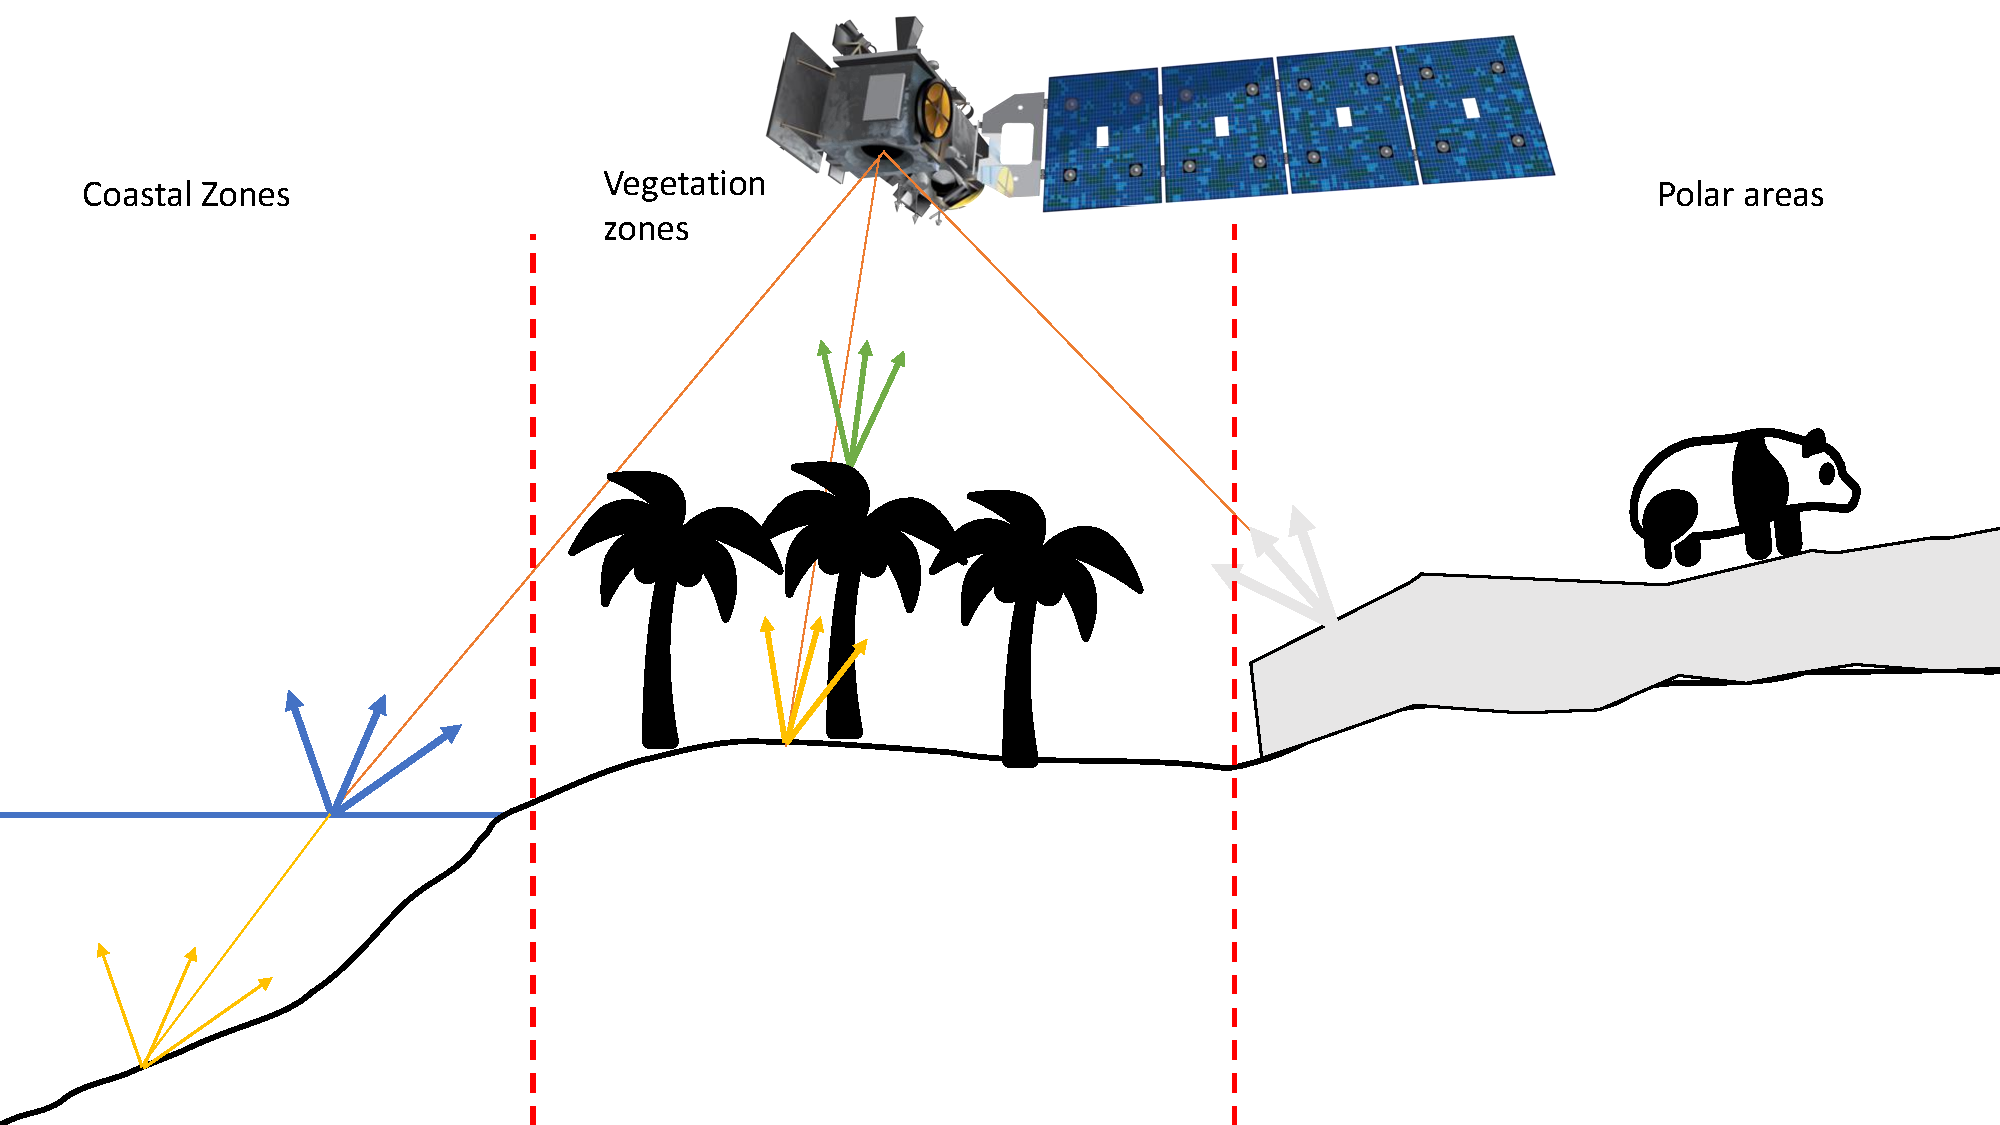
\includegraphics[width=0.75\textwidth]{figures/summary.pdf}
      % \caption{Overview}\pdfcomment{obviously this is a pretty rough draft ;) }
      \label{fig:icesat-summary-image}
  \end{figure}
  

\section{Research Question}
The primary question that this project intends to answer is: \\
\\
\textit{How can spaceborne remote sensing data be combined with existing global datasets to improve estimates of nearshore bathymetry?} 

To answer this question, the following subquestions will be investigated:

\begin{enumerate} 
      \item How can ICESat-2 transects that contain bathymetry be identified algorithmically?
      \item Once transects with bathymetry are found, how can nearshore subsurface photon returns that are located in the nearshore zone be extracted?
      \item How can lidar photon return locations reflecting the seafloor be separated from background noise?
      \item What is the potential to scale up bathymetry detection to a global scale to produce high-level processed bathymetry product using ICESat-2 data?
      \item How can spaceborne remote sensing sources be used to improve existing global bathymetry datasets?
      \item Under what conditions can remotely-sensed lidar data provide useful improvement on bathymetric data estimates?
\end{enumerate}
